% vim: textwidth=110
% Suppress some acceptable compilation warnings
\RequirePackage[save,showerrors]{silence}
\WarningFilter{transparent}
  {Loading aborted} % Used (or at least tried) by the svg package
\WarningFilter{multicol}
  {May not work with the twocolumn option} % I'm not really using the multicol package
\WarningFilter{latex}
  {Marginpar on page} % Margin stuff moved to not overlap with other stuff, this is fine
\WarningFilter{caption}
  {Unknown document class} % the caption package doesn't know about llncs

% llncs class documentation:
% https://ctan.tetaneutral.net/macros/latex/contrib/llncs/llncsdoc.pdf
\documentclass[dvipsnames,runningheads]{llncs}

% language settings
\usepackage[main=french,english]{babel}
\newcommand{\en}[1]{\foreignlanguage{english}{\emph{#1}}}
\usepackage{csquotes}
\MakeOuterQuote{"}
% Fix LLNCS language handling of the "keywords" part of the abstracts
\addto{\captionsfrench}{\renewcommand{\keywordname}{\textbf{Mots-clé:}}}

% Hyphenation
\hyphenation{Git-Hub}

% links setup
\usepackage[nobiblatex]{xurl}
\usepackage{hyperref}
\hypersetup{colorlinks=true}

% bibliography settings
\usepackage[hyperref=true,isbn=false,eprint=false,giveninits=true]{biblatex}
% redefine the "title" field style to remove quotation marks
\DeclareFieldFormat*{title}{#1}
% redefine the "url" field to remove protocol information (https://)
\DeclareSourcemap{
    \maps[datatype=bibtex]{
        \map{
            \step[fieldsource=url, final=true]
            \step[fieldset=verba, origfieldval, final=true]
            \step[fieldsource=verba, match=\regexp{\A(ht|f)tp(s)?:\/\/}, replace={}]
        }
    }
}
\DeclareFieldFormat{url}{%
    \mkbibacro{URL}\addcolon\space
    \href{#1}{\nolinkurl{\thefield{verba}}}%
}
\DefineBibliographyExtras{french}{\restorecommand\mkbibnamefamily}
\addbibresource{../references.bib}

% Hypotheses
\newtheorem{hypo}{Hypothèse}[theorem]

% For file inclusion and figure formatting
\usepackage{caption}
\usepackage{subcaption}

% Other
\usepackage{todonotes}
\usepackage{mathtools}

\title{L'Identification des Projets de Logiciel Libre Accessibles aux Nouveaux Contributeurs}
\titlerunning{Projets de Logiciel Libre Accessibles aux Nouveaux Contributeurs}
% TODO: de-anonymize authors
\author{%
    Premier Auteur\inst{1}%Paul Hervot\inst{1}%
    \and%
    Deuxième Auteur\inst{2}%Benoît Crespin\inst{2}\orcidID{0000-0002-9105-0243}%
}
% TODO: de-anonymize institutions
\institute{Institution du premier auteur \and institution du deuxième auteur} %\institute{EPITA \and Université de Limoge}
% hack the "short author" mecanism to display the conference name on even pages instead
\authorrunning{Environnements Informatiques pour l’Apprentissage Humain 2023}

\begin{document}
    \maketitle

    % Abstracts and keywords
    \selectlanguage{french}
    \begin{abstract}
        Le logiciel libre prend de plus en plus de place dans le paysage public et industriel, notamment pour
        sa transparence et sa gestion démocratique, pour autant publier le code source d'un logiciel ne le
        rend pas automatiquement accessible, et les nouveaux contributeurs de ces projets rencontrent de
        nombreuses barrières les entravant dans leurs contributions. Au travers d'une analyse à grande échelle
        de l'archive de Software Heritage, nous testons la pertinence de trois indicateurs dans
        l'identification des logiciels libres accessibles aux nouveaux contributeurs. Nos résultats montrent
        une corrélation positive entre le nombre de premières contributions réussies dans un projet et la
        présence d'instructions de contribution, ainsi qu'entre ce même nombre et celui des contributeurs
        uniques récents du projet. Ces indicateurs trouveront une utilité dans l'enseignement des pratiques du
        logiciel libre, les enseignants de ce sujet rencontrant des difficultés à sélectionner des projets
        accessibles sur lesquels faire travailler leurs étudiants.

        \keywords{
            Collecte, traitement et analyse des traces d’apprentissage \and
            Analyse d’usage(s) et de pratiques \and
            Logiciel libre \and
            Analyse automatique de dépôts logiciels \and
            Barrières d'entrée du logiciel libre
        }
    \end{abstract}
    \selectlanguage{english}
    \begin{abstract}
        FOSS makes an increasing amount of the public and industrial software landscape, notably for its
        transparency and democratic governance. However, simply publishing the source code of a software does
        not automatically make it accessible, and many barriers impede new contributors approaching these
        projects. Through a large-scale software mining of the Software Heritage archive, we test the
        pertinence of three signals in the identification of accessible FOSS projects for new contributors.
        Our results show a positive correlation between the number of new contributors of a project
        successfully bringing their contribution to completion and the presence of contributing guidelines, as
        well as between that same number and the number of recent unique contributors in the project. Such
        signals could find a use in the teaching of FOSS practices, as teachers of this subject often find it
        difficult to select an accessible project for their students to work on.

        \keywords{
            Collection, processing and analysis of learning traces \and
            Usage and practices analysis \and
            FOSS \and
            Mining Software Repositories \and
            Open source barriers to entry
        }
    \end{abstract}
    \selectlanguage{french}

    \section{Introduction}

    Quelques initiatives existent pour enseigner les pratiques du logiciel libre dans l'éducation supérieur et
    la formation professionnelle, mais elles sont rares. Certaines viennent des communautés du logiciel libre,
    comme le
    \href{https://www.edx.org/professional-certificate/linuxfoundationx-open-source-software-development-linux-and-git}{\en{Professional
    Certificate in Open Source Software Development, Linux and Git}} de la \en{Linux Foundation}, ou les
    séminaires de l'\href{https://opensource.org/osi-open-source-education}{\en{open source initiative}}.
    Certaines universités proposent des cursus en informatique abordant les pratiques du logiciel libre, comme
    l'Université de l'État de Caroline du Nord aux États-Unis \parencite{oss-edu-2008} ; ou
    l'université de Calais qui propose actuellement un
    \href{https://www.univ-littoral.fr/formation/offre-de-formation/masters/master-informatique-ingenierie-du-logiciel-libre/}{Master
    Informatique - Ingénierie du logiciel libre} en alternance.

    Ces initiativent incluent toutes une part de pédagogie de projet, méthode à laquelle plusieurs
    méta-analyses attribuent d'importants effets positifs \cite{pbl-2019, pbl-2018}. Les projets proposés aux
    étudiants sont cependant souvent factices, créés par les enseignants dans le seul but de servir
    d'exercice. Utiliser au contraire des projets réels, qui ne cessent pas d'exister après la fin de la
    séquence pédagogique, donne des résultats encore meilleurs, mais est aussi plus incertain à mettre en
    place \cite{real-pbl-2010, real-pbl-2004}. Certains compromis on été tentés, consistant à créer des
    projets proches de situations réelles, mais dédiés à l'éducation \cite{oss-edu-2008}. Ces projets ne sont
    cependant plus accessibles aujourd'hui, possiblement à cause de leur portée réduite à l'éducation et à
    l'absence d'une communauté persistante autour d'eux.

    \section{Nouveaux contributeurs}

    \textcite{barriers-2018} notent la difficulté des nouveaux volontaires à rejoindre une communauté de
    logiciel libre, citant comme exemple extrême le projet Apache Hadoop qui a vu 82\% de ses nouveaux
    volontaires quitter le projet après leur première contribution \parencite{hadoop-dropout-2013}. Une des
    tendances qu'ils trouvent est que la majorité ($58\%$) des barrières rencontrées dans leur étude sont de
    nature sociale et non techniques \parencite[p.~1008]{barriers-2018}. Il semble en outre que les outils et
    la documentation représentent la majorité des barrières techniques rencontrées, éléments ayant
    paradoxalement pour objectif d'aider les nouvelles contributions. Ce frein semble empirer lorsque les
    méthodes d'apprentissage et de traitement de l'information de la personne consistent à rassembler le plus
    d'information possible avant de commencer à agir. Ces méthodes étant sur-représentées chez les femmes
    \parencite{gender-information-processing-1995,gender-information-processing-2015}, ces barrières
    deviennent discriminantes selon le genre, et peuvent participer à expliquer la sous-représentation des
    femmes dans les communautés de logiciel libre.

    \label{sec:accessibility-measure}
    Plusieurs mesures \emph{a posteriori} de l'accessibilité des projets de logiciel libre ont été faites, en
    majorité de façon qualitative \parencites{newcomers-accessibility-2016}{newcomers-onboarding-2018}[voir
    aussi][]{newcomers-adaptation-2005}. Une approche quantitative encore rare consiste à étudier la
    progression du nombre total de contributeurs au cours de la vie du projet \cite{contributor-count-2006}.
    Similairement, \textcite{signals-2019} étudient les signaux que les potentiels nouveaux contributeurs
    observent pour choisir un projet auquel contribuer. Ils s'intéressent pour cela spécifiquement aux projets
    disponibles publiquement sur \en{github}, ce qui leur permet d'étudier empiriquement l'effet des signaux
    que la plateforme met en évidence. Ils suggèrent qu'une mesure possible de l'accessibilité pour les
    nouveaux contributeurs ("\en{newcomers openness}" dans l'article) est le pourcentage de \en{pull requests}
    créées par des contributeurs externes, qu'ils définissent par opposition aux \en{core contributors} : les
    personnes auteurs de plus de 5\% des \en{commits} du projet. En réalité cependant, leur étude ne retient
    que la présence ou non de \en{pull request} venant de nouveaux contributeurs (p.~16), ce qui leur permet
    de n'étudier qu'une variable binaire.

    Pour leur analyse quantitative, \textcite{signals-2019} collectent leurs données via l'\en{API} de GitHub,
    comme beaucoup d'études récentes \parencite{github-mapping-2017}. La plateforme est très populaire dans le
    milieu du logiciel libre, mais ces mêmes études notent cependant que se restreindre à cette seule
    plateforme limite la représentativité des données étudiées \parencite{swh-growth-2019}. Les limites et
    erreurs courantes liées au minage de GitHub font d'ailleurs l'objet d'une littérature grandissante et
    remettant en question certains résultats utilisant cette technique sans détailler suffisamment leur
    méthodologie \parencite{mining-github-2014,penumbra-oss-2022}. \textcite{barriers-meta-2015} remarquent de
    plus que dans la littérature, les études se concentrent trop sur les projets importants et matures, un
    biais permettant d'obtenir une quantité importante de données mais ignorant une grande part du logiciel
    libre. À l'inverse, 71\% des projets hébergés sur GitHub sont des projets personnels et non réellement
    collaboratifs, c'est pourquoi \textcite{mining-github-2014} ne retiennent pour leur étude que ceux ayant
    au moins deux auteurs uniques différents.

    Il faut donc approfondir la recherche dans cette direction, mais le nombre de projets et des artéfacts qui
    leur sont liés augmente exponentiellement \parencite{swh-growth-2019}, avec un phénomène de duplication :
    des fichiers identiques se retrouvent dans de nombreux projets différents (comme les notices de licence).
    Beaucoup de \en{commits} eux-même peuvent se trouver dans plusieurs projets différents après un \en{fork}.
    L'analyse à grande échelle de l'historique de développement des projets de logiciel libre devient donc de
    plus en plus complexe à implémenter efficacement.

    \section{L'archive de logiciels de Software Heritage}

    \label{ssec:swh-graph}

    Les techniques de compression de graphe sont aujourd'hui suffisamment avancées pour permettre une nouvelle
    approche à cette analyse automatique des projets, en les rassemblant au sein d'une même structure de
    donnée unifiée et optimisée \parencite{swh-graph-2020}. La structure de donnée proposée par
    \textcite{swh-graph-2020} est un graphe orienté où chaque \en{commit} est représenté par un nœud et où
    chaque arc $u \xrightarrow{succ} v$ ("le \en{commit} $v$ est un ancêtre immédiat de $u$") possède aussi un
    arc inverse $u \xleftarrow{pred} v$. Cette structure permet donc de trouver tous les \en{fork} d'un
    projet avec un classique calcul de composante fortement connexe.

    Software Heritage est une initiative exploitant ces techniques de compression afin de construire une
    archive aussi complète que possible du code source actuellement disponible publiquement dans le monde.
    L'archive est publique et se veut exploitable pour la recherche \parencite{swh-2017}. Il s'agit du corpus
    que \textcite{swh-graph-2020} ont utilisé comme exemple pour leur modèle de compression. L'archive
    comptait en 2018 plus d'un milliard de \en{commits} uniques archivés depuis 85 millions d'origines
    différentes (\en{remotes} \en{git}, paquets \href{https://pypi.org/}{PyPi}, etc.). L'archive grandit de
    façon continue en ajoutant petit à petit de nouveaux projets et de nouveaux artéfacts à chaque évolution
    des projets déjà archivés, ce qui en fait l'un des corpus les plus complets et exploitables par la
    recherche scientifique \parencite{swh-2019,swh-growth-2019}.

    \section{Méthodologie}

    \subsection{Problématique}

    La question de l'accessibilité des projets de logiciel libre pour les nouveaux contributeurs est encore
    assez peu explorée de façon quantitative dans la littérature. \textcite{signals-2019} se sont intéressés
    aux signaux que les potentiels nouveaux contributeurs observent pour choisir un projets auquel
    \emph{essayer} de contribuer, nous proposons de déterminer si certains de ces signaux sont de surcroit
    prédictifs d'une réelle accessibilité de ces projets, c'est à dire à quel point de nouveaux contributeurs
    \emph{réussissent} à produire une contribution apparaissant dans l'historique de développement du projet.
    Pour dépasser les limitations de GitHub, nous utiliserons l'archive de Software Heritage comme accès à la
    population étudiée. Ce choix nous empêchera cependant d'étudier les indicateurs propres à GitHub comme le
    nombre de \en{pull requests} d'un projet.

    Pour évaluer l'accessibilité d'un projet, nous proposons d'utiliser comme variable proxy le nombre de
    contributeurs apparaissant pour la première fois dans l'historique de développement du projet entre le
    premier juin 2019 et le premier septembre 2019 \parencite[voir section \ref{sec:accessibility-measure},
    ainsi que][p.~13,16]{signals-2019}. Cette période de référence a été choisie sur recommandation de
    Software Heritage, la désignant comme un bon compromis entre le nombre de projets pour lesquels les
    données sont disponible dans l'archive et le caractère récent des observations.

    Nous souhaitons tester trois hypothèses reprenant celles de \textcite[voir p.~11-13 et 16]{signals-2019}.
    Nous considérons comme "récent" tout événement survenu dans les six mois avant la période de référence
    étudiée.

    \newcommand{\newhyp}[2]{%
        \begin{hypo}
            \label{hyp:#1}: #2
        \end{hypo}%
    }

    \newhyp{contributionguidelines}{%
        les projets possédant des instructions de contribution sont plus accessibles pour les nouveaux
        contributeurs que ceux n'en ayant pas.%
    }

    \newhyp{recentcontributorcount}{%
        le nombre de contributeurs uniques récents d'un projet est positivement corrélée à son accessibilité
        pour les nouveaux contributeurs.%
    }

    \newhyp{recentcommitcount}{%
        le nombre de \en{commits} récents au sein d'un projet est positivement corrélé à son accessibilité
        pour les nouveaux contributeurs.%
    }

    \subsection{Échantillon et collecte initiale}
    \label{sec:constitution_echantillon}

    Plusieurs critères d'exclusion ont été appliqués sur l'archive de Software Heritage pour constituer notre
    échantillon :

    \begin{itemize}
        \item quand plusieurs projets ont des \en{commits} en commun et sont donc des \en{forks} les uns des
            autres, seul celui qui la plus longue chaîne de \en{commits} a été retenu comme représentant du
            groupe ;
        \item sont exclus pour inactivité les projets n'ayant reçu aucun \en{commit} pendant la période de
            référence \parencite[voir][]{mining-github-2014} ;
        \item sont exclus pour caractère non-collaboratif les projets ayant vu moins de deux
            contributeurs uniques récents \parencite[voir][]{mining-github-2014}.
    \end{itemize}

    Un nœud du graphe de l'archive de Software Heritage peut représenter un \en{commit} ("\en{revisions}"),
    une origine (l'URL à partir de laquelle a été archivé un projet), un \en{snapshot} (point de départ daté
    d'une passe d'archivage), un dossier ou un fichiers. Un arc $u \xrightarrow{succ} v$ peut donc signifier,
    en fonction des types de $u$ et $v$, que : 

    \begin{itemize}
        \item $u$ est un \en{commit} successeur du \en{commit} $v$ ;
        \item $v$ est un \en{snapshot} du projet disponible à l'origine $u$ ;
        \item $v$ est le dernier \en{commit} d'une des branches visibles lors du \en{snapshot} $u$ ;
        \item $v$ est le dossier racine du contenu du projet en l'état du \en{commit} $u$ ;
        \item etc.
    \end{itemize}

    Nous effectuons un premier parcours du graphe à partir de chaque origine afin d'identifier le représentant
    de chaque groupe de fork (composante fortement connexe sur les liens entre \en{commits}). Un parcours
    largeur avec marqueurs de niveaux en remontant des \en{commits} initiaux vers les origines qui lui sont
    accessibles permet d'identifier la plus longue chaîne de \en{commits} et donc le représentant de son
    groupe de \en{fork}. Pour le \en{snapshot} le plus récent de chaque origine ainsi retenue, un nouveau
    parcours est effectué à partir de sa branche principale afin de récolter les données de recherche. Le
    nombre de contributeurs et de \en{commits} récents se compte facilement lors du parcours, mais la présence
    d'instructions de contribution est plus difficile à vérifier car le graphe ne contient que les noms et la
    hierarchie des fichiers d'un projet, mais pas leur contenu. Ce parcours ne vérifie donc initialement que
    la présence d'un fichier \texttt{CONTRIBUTING.md} ou assimilé, auquel cas nous validons la présence
    d'instructions de contribution. En son absence, nous vérifions la présence d'un fichier \texttt{README.md}
    ou assimilé, en cas de deuxième absence nous validons l'\emph{absence} d'instructions de contribution. En
    présence d'un \texttt{README}, nous sauvegardons l'identifiant unique du fichier afin d'analyser son
    contenu ultérieurement. Enfin, le nombre de nouveaux contributeurs est calculé en comptant les
    contributeurs uniques de la période de référence qui n'apparaissent dans aucun \en{commit} antérieur à
    cette période.

    \label{sec:collectreadme}
    Restent à traiter certains \texttt{README}. Leur contenu peut être téléchargé publiquement soit via des
    requêtes HTTP sur le site \href{https://archive.softwareheritage.org/}{archive.softwareheritage.org}, soit
    depuis le \en{registry} Amazon S3
    \href{https://registry.opendata.aws/software-heritage}{software-heritage}. Le site limite le nombre de
    requêtes autorisées par adresse IP à quelques dizaines par heure, contrairement au \en{registry}, mais ce
    dernier ne contient pas encore tous les contenus archivés. Nous téléchargeons donc en priorité via le
    \en{registry} Amazon S3 et nous rabattons sur le site pour les fichiers manquants. Nous cherchons ensuite
    dans ces \texttt{README} une section contenant le mot \en{contributing} ou une expression proche. Les noms
    de sections sont identifiés en supposant que les \texttt{README} sont formattés en Markdown ou
    reStructuredText et en se basant sur leur syntaxe officielle \parencite{markdown-headings,rst-sections}.

    Un \en{replication package} contenant le code source et les bibliothèques utilisés dans ce mémoire, ainsi
    que les données brut collectées, a été publié sur Zenodo
    \parencite[anonymisé]{anonymous-replication-package}.
    % TODO: de-anonymize and upload new version to zenodo

    \section{Résultats et discussion}

    % Figure caption setup
    \captionsetup[figure]{format=plain,singlelinecheck=true,justification=centering}
    \captionsetup[subfigure]{format=plain,singlelinecheck=true,justification=centering}
    \captionsetup[table]{format=plain,singlelinecheck=true,justification=centering,position=above}

    \begin{table}[ht]
        \centering
        \caption{Aperçu statistique des données collectées}
        \begin{tabular}{c|c}
            \begin{tabular}{ll}
 & hasContrib \\
count & 27619 \\
unique & 2 \\
top & no \\
freq & 23740 \\
\end{tabular}
 &
            \begin{tabular}{lr}
 & \textbf{recentCommitCount} \\
count & 60966.00 \\
mean & 61.79 \\
std & 408.96 \\
min & 2.00 \\
25\% & 8.00 \\
50\% & 19.00 \\
75\% & 49.00 \\
max & 36176.00 \\
\end{tabular}
\\
            \hline
            \\
            \begin{tabular}{lr}
 & \textbf{recentContributorCount} \\
count & 60966.000000 \\
mean & 3.246268 \\
std & 6.983897 \\
min & 2.000000 \\
25\% & 2.000000 \\
50\% & 2.000000 \\
75\% & 3.000000 \\
max & 688.000000 \\
\end{tabular}
 &
            \begin{tabular}{lr}
 & newContributorCount \\
count & 60966.000000 \\
mean & 0.522209 \\
std & 1.663200 \\
min & 0.000000 \\
25\% & 0.000000 \\
50\% & 0.000000 \\
75\% & 1.000000 \\
max & 130.000000 \\
\end{tabular}

        \end{tabular}
        \label{tab:data_description}
    \end{table}

    Sur les $60 966$ projets distincts (sans historique commun) analysés, $14\%$ d'entre eux possèdent des
    instructions de contribution. Les nombres de \en{commits} récents, de contributeurs récents et de nouveaux
    contributeurs varient fortement au sein de cette population, la distribution n'est normale dans aucun des
    deux cas (voir figure \ref{fig:distribution}).

    \begin{figure}[ht]
        % Distribution
        \begin{subfigure}[t]{0.333\textwidth}
            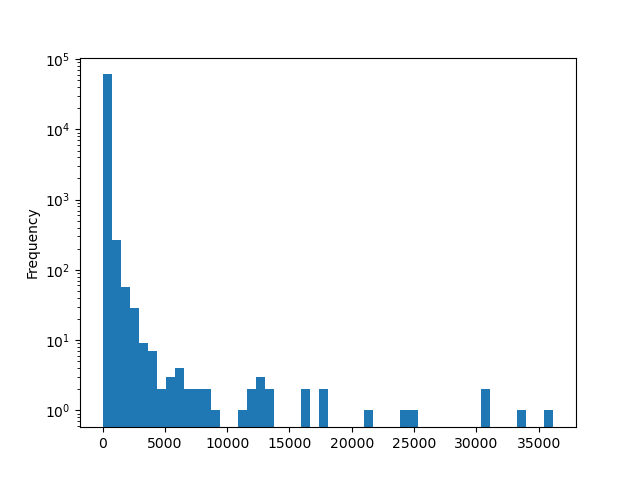
\includegraphics[width=\textwidth]{../experiment/data_analysis/recentCommitCount_distribution}
            \caption{\en{Commits} récents (distribution)}
        \end{subfigure}
        \begin{subfigure}[t]{0.333\textwidth}
            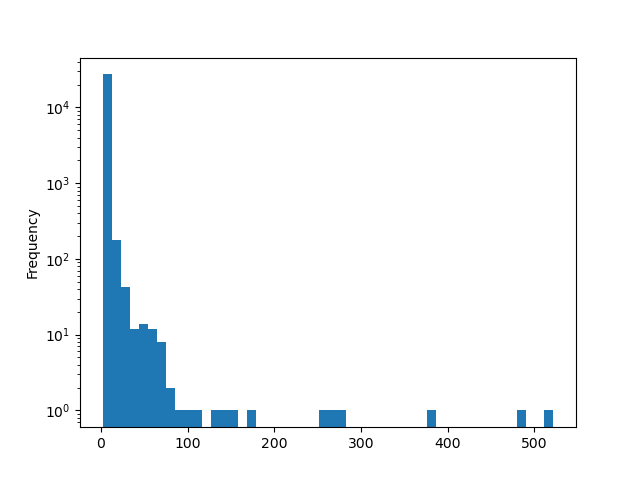
\includegraphics[width=\textwidth]{../experiment/data_analysis/recentContributorCount_distribution}
            \caption{Contributeurs récents (distribution)}
        \end{subfigure}%
        \begin{subfigure}[t]{0.333\textwidth}
            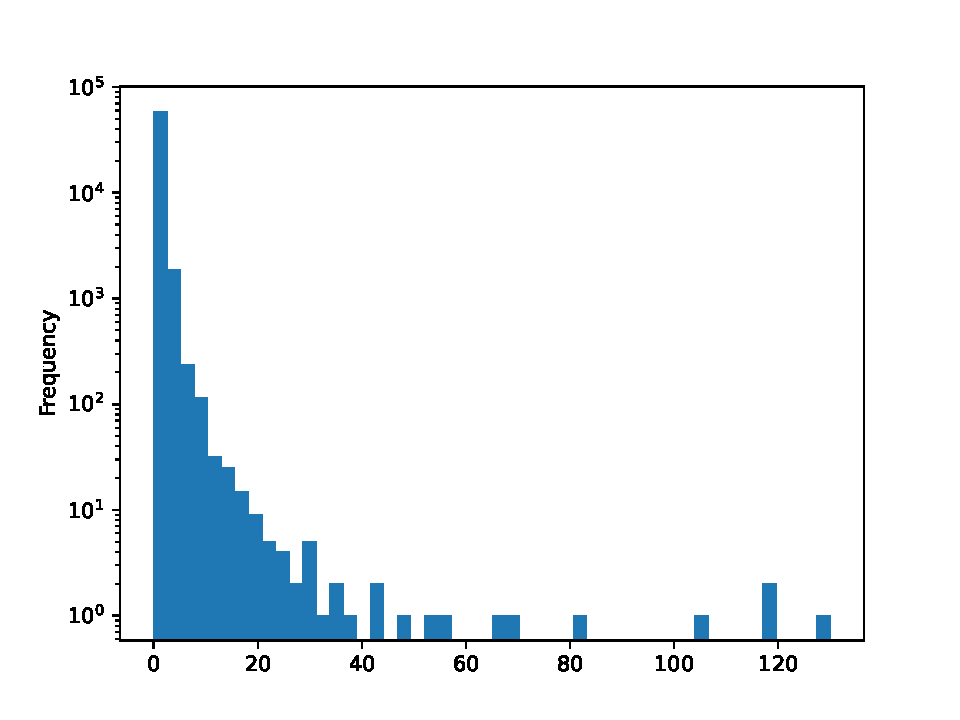
\includegraphics[width=\textwidth]{../experiment/data_analysis/newContributorCount_distribution}
            \caption{Nouveaux contributeurs (distribution)}
        \end{subfigure}

        % QQ-plots
        \begin{subfigure}[t]{0.333\textwidth}
            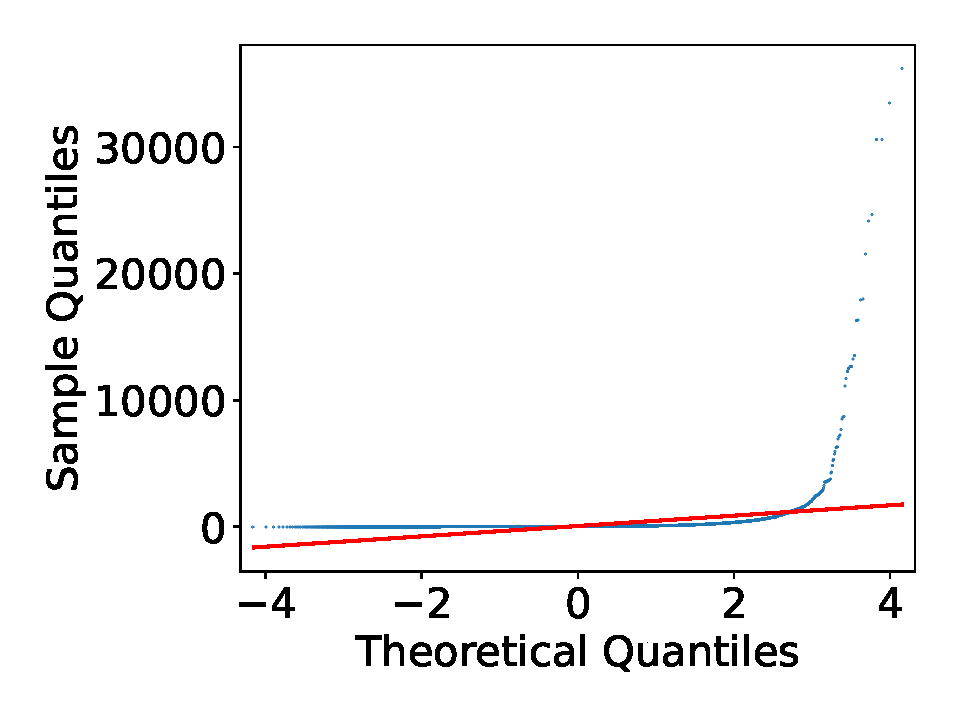
\includegraphics[width=\textwidth]{../experiment/data_analysis/recentCommitCount_qqplot}
            \caption{\en{Commits} récents (qq-plot)}
        \end{subfigure}
        \begin{subfigure}[t]{0.333\textwidth}
            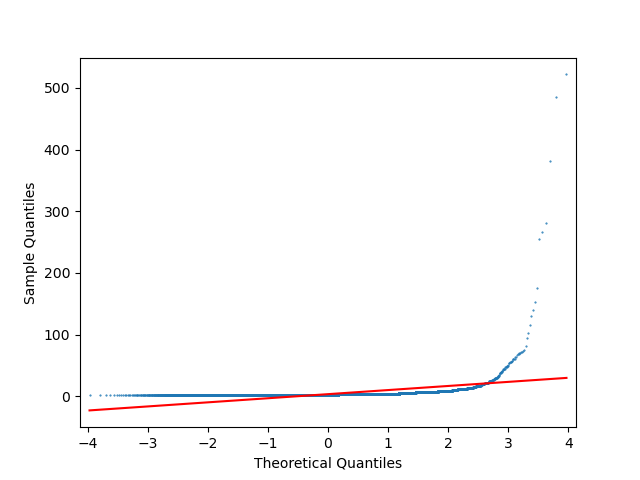
\includegraphics[width=\textwidth]{../experiment/data_analysis/recentContributorCount_qqplot}
            \caption{Contributeurs récents (qq-plot)}
        \end{subfigure}%
        \begin{subfigure}[t]{0.333\textwidth}
            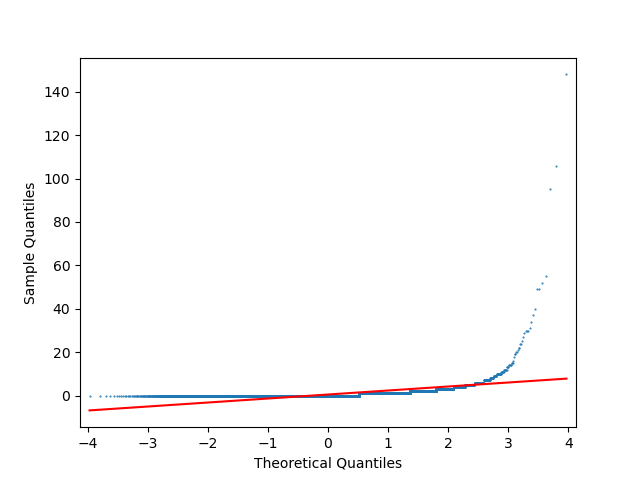
\includegraphics[width=\textwidth]{../experiment/data_analysis/newContributorCount_qqplot}
            \caption{Nouveaux contributeurs (qq-plot)}
            \label{sfig:newContributorQQplot}
        \end{subfigure}

        \caption{%
            Distribution (avec ordonnée logarithmique) et diagrammes quantile-quantile pour variable
            numérique%
        }
        \label{fig:distribution}
    \end{figure}

    \begin{figure}[ht]
        \begin{subfigure}[t]{0.5\textwidth}
            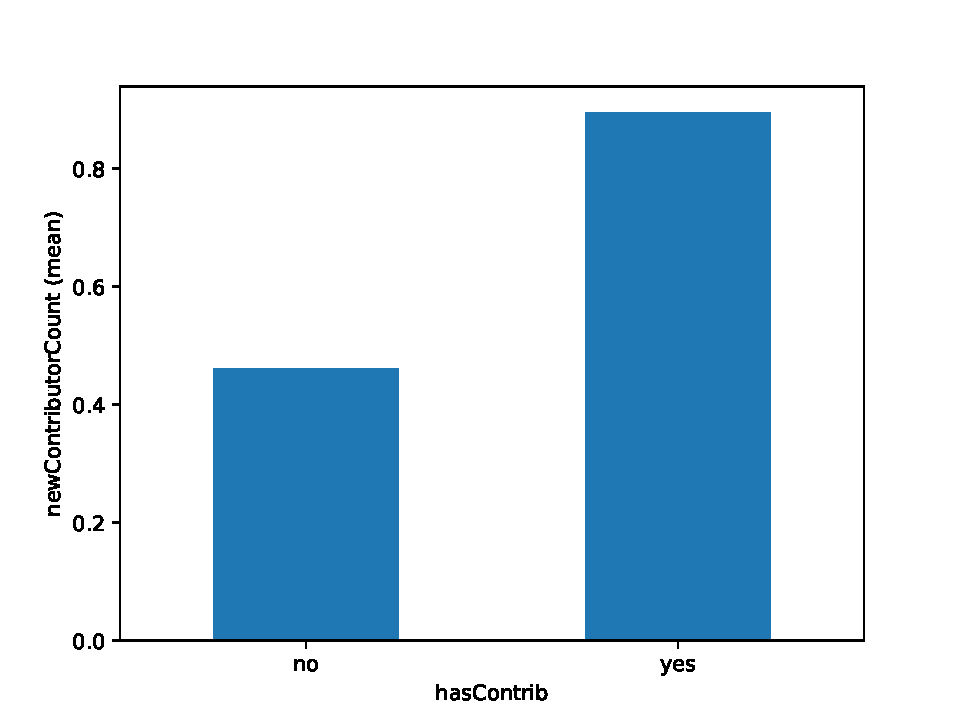
\includegraphics[width=\textwidth]{../experiment/data_analysis/hasContrib_meanNewContributorCount}
            \caption{Moyenne}
        \end{subfigure}%
        \begin{subfigure}[t]{0.5\textwidth}
            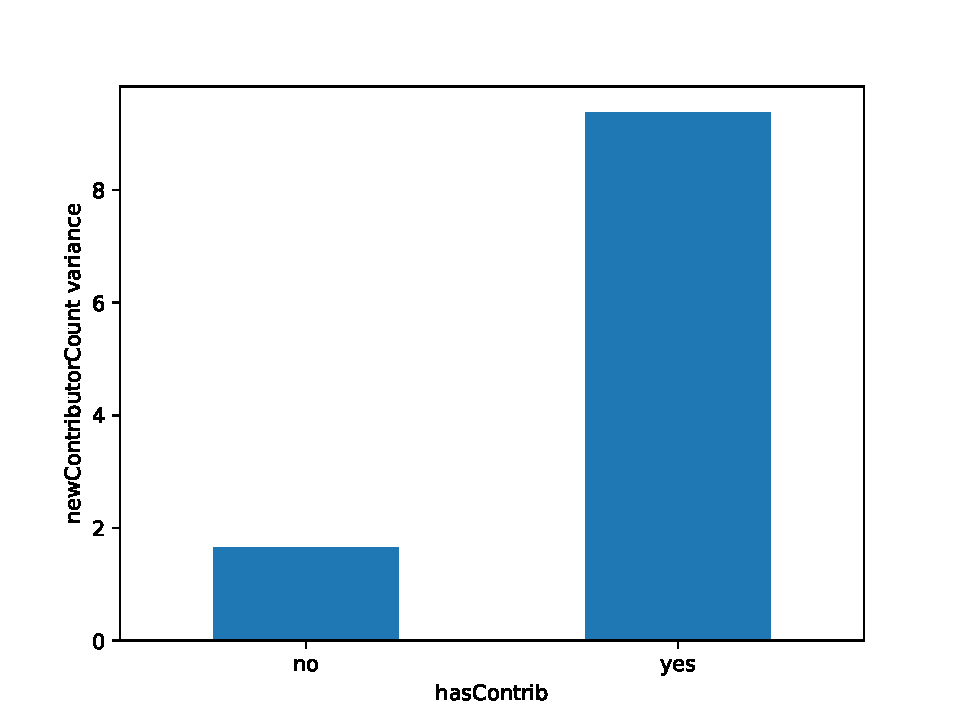
\includegraphics[width=\textwidth]{../experiment/data_analysis/hasContrib_varianceNewContributorCount}
            \caption{Variance}
            \label{sfig:hasContribVariance}
        \end{subfigure}

        \caption{Moyenne et variance du nombre de nouveaux contributeurs pour chaque catégorie}
        \label{fig:hasContrib}
    \end{figure}

    Les projets possédant des instructions de contribution ont en moyenne plus de nouveaux contributeurs (voir
    figure \ref{fig:hasContrib}), un test de Wilcoxon-Mann-Whitney donne une taille d'effet $\rho \approx
    0.57$ et confirme ($p \approx 0$) que les deux distribution sont bien différente. L'hypothèse du test
    étant que les projets avec instructions de contribution ont un meilleur score que les autres
    (contrairement à la version \en{two-tailed}), nous pouvons valider
    \hyperref[hyp:contributionguidelines]{l'hypothèse H\ref*{hyp:contributionguidelines}}. Ce résultat est
    cohérent avec ceux de \textcite[p.~11]{signals-2019}. De futures recherches pourraient essayer de
    déterminer si ce plus grand nombre de nouveaux contributeurs \emph{ayant réussi} à contribuer est dû
    uniquement à ce plus grand nombre de nouveaux contributeurs \emph{essayant} de contribuer, ou si la
    présence d'instructions de contribution a un réel rôle dans le succès d'une tentative de contribution. Il
    est tout de même important de noter que, bien que le test de Wilcoxon-Mann-Whitney ne soit pas
    paramétrique et puisse donc s'appliquer à ces données, sa robustesse diminue significativement lorsque la
    distribution des données ne suit pas une loi normale \emph{et} que les groupes comparés ont une variance
    significativement différente \parencite{WMW-robustness-1998}, ce qui est le cas ici (voir figures
    \ref{sfig:newContributorQQplot} et \ref{sfig:hasContribVariance}). Ce point, ainsi que la petite taille
    d'effet obtenue, justifieraient une attention plus particulière à la collecte et préparation des données
    afin d'approcher une distribution normale et d'en homogénéiser la variance.

    \begin{figure}
        \centering
        \begin{subfigure}[t]{0.5\textwidth}
            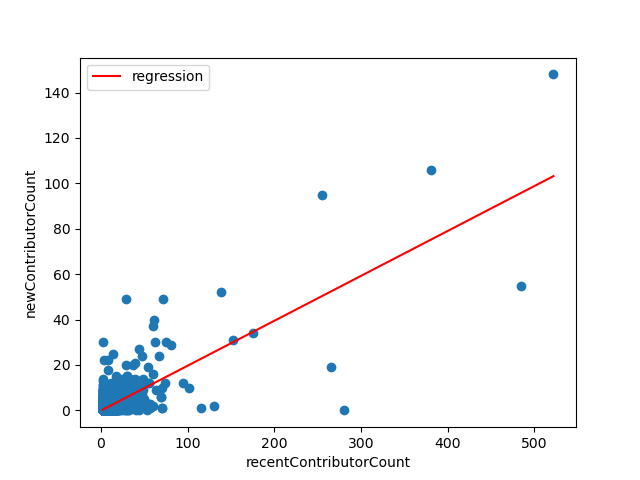
\includegraphics[width=\textwidth]{../experiment/data_analysis/recentContributorCountRegression_linearScale}
            \caption{Échelle linéaire}
        \end{subfigure}%
        \begin{subfigure}[t]{0.5\textwidth}
            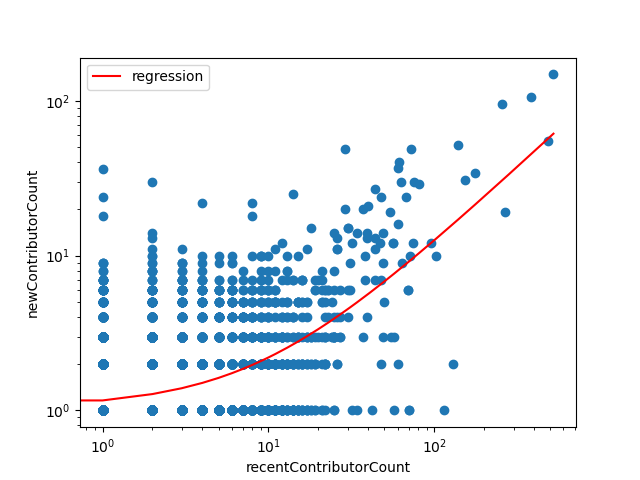
\includegraphics[width=\textwidth]{../experiment/data_analysis/recentContributorCountRegression_logScale}
            \caption{Échelle logarithmique}
        \end{subfigure}

        \caption{Nombre de nouveaux contributeurs en fonction du nombre de contributeurs uniques récents}
        \label{fig:contributorCount}
    \end{figure}

    \begin{figure}[ht]
        \centering
        \begin{subfigure}[t]{0.5\textwidth}
            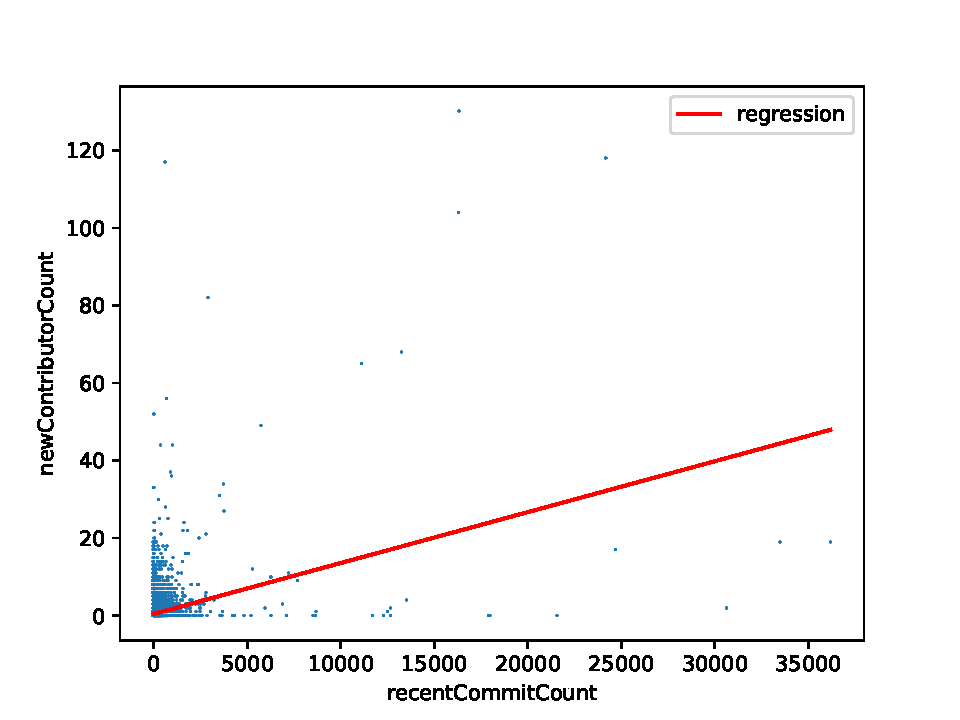
\includegraphics[width=\textwidth]{../experiment/data_analysis/recentCommitCountRegression_linearScale}
            \caption{Échelle linéaire}
        \end{subfigure}%
        \begin{subfigure}[t]{0.5\textwidth}
            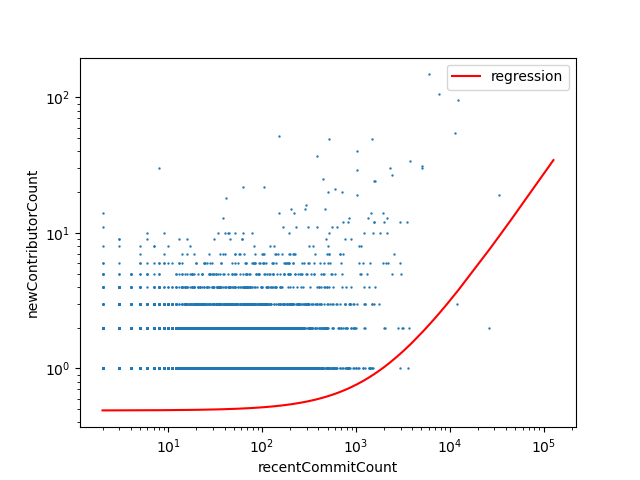
\includegraphics[width=\textwidth]{../experiment/data_analysis/recentCommitCountRegression_logScale}
            \caption{Échelle logarithmique}
        \end{subfigure}

        \caption{Nombre de nouveaux contributeurs en fonction du nombre de \emph{commits} récents}
        \label{fig:commitCount}
    \end{figure}

    Un premier modèle de régression linéaire utilisant la méthode des moindres carrés ordinaires a été calculé
    pour comparer le nombre de contributeurs récents avec celui des nouveaux contributeurs
    (Fig.~\ref{fig:contributorCount}). Un test d'homoscédasticité de White revèle une forte hétéroscédasticité
    des données de la régression ($p = 0$), ce qui implique que la méthode OLS n'est pas la plus
    statistiquement efficace pour modéliser la relation entre les deux variables \parencite{GLS-2021}. Le
    modèle retenu utilise donc la méthode des moindres carrés généralisée (modèle
    \href{https://www.statsmodels.org/dev/generated/statsmodels.regression.linear_model.GLS.html}{GLS} du
    paquet Python \texttt{statsmodel}), il suggère effectivement que plus le nombre de contributeurs récents
    d'un projet est élevé, plus son nombre de nouveaux contributeurs l'est aussi. Le coefficient de
    détermination $R^2 \approx 0.45$ du modèle indique que le nombre de contributeurs récents explique environ
    $45\%$ de la variation du nombre de nouveaux contributeurs, ce qui valide
    \hyperref[hyp:recentcontributorcount]{l'hypothèse H\ref*{hyp:recentcontributorcount}}, avec une taille
    d'effet tout de même modérée. Ce résultat est aussi cohérent avec ceux de
    \textcite[p.~12-13,16]{signals-2019} qui observaient que le nombre de contributeurs uniques récents était
    positivement corrélé au nombre de \emph{tentatives} de contribution faites par de nouveaux contributeurs
    (mesuré par le nombre de \en{pull requests}). Là aussi de futures recherches pourraient s'intéresser à la
    causalité de cette relation. Tout ce que notre étude peut affirmer sur un éventuel lien de causalité est
    que, le nombre de contributeurs récents étant mesuré sur une période antécédente à celle sur laquelle est
    mesuré le nombre de nouveaux contributeurs, cette deuxième variable ne peut pas influencer la première.

    Suivant la même approche pour l'analyse du nombre de \en{commits} récents, une première régression avec la
    méthode des moindres carrés ordinaires a d'abord été faite, puis écartée par un test d'homoscédasticité de
    White. C'est donc une régression linéaire utilisant la méthode des moindres carrés généralisée qui a été
    retenue (Fig.~\ref{fig:commitCount}). Le modèle suggère ici aussi une corrélation positive entre le nombre
    de \en{commits} récents d'un projet et son nombre de nouveaux contributeurs, mais son coefficient de
    détermination est trop faible ($R^2 \approx 0.10$) pour considérer que le modèle représente fidèlement des
    données du problème. Nous ne pouvons donc conclure à une relation entre ces deux variables et devons
    rejeter \hyperref[hyp:recentcommitcount]{l'hypothèse H\ref*{hyp:recentcommitcount}}. Ce résultat ne
    rejoint cette fois pas ceux de \textcite[p.~13,16]{signals-2019}. Cela pourrait signifier que le nombre de
    \en{commits} récents d'un projet est un signal que les nouveaux contributeurs potentiels utilisent \emph{à
    tort} pour choisir un projet auquel essayer de contribuer. Nos résultats ne permettent pas de conclure
    qu'un grand nombre de \en{commits} récents, bien qu'il attire les nouveaux contributeurs, est un
    indicateur de l'accessibilité du projet pour ces nouveaux contributeurs.

    \section{Conclusion}

    Par l'analyse de l'archive de Software Heritage, l'un des corpus de développement logiciel les plus
    représentatifs et exploitables dans un contexte de recherche, nous avons tenté de déterminer si trois
    signaux facilement observables pour un enseignant ou un nouveau contributeur sont prédictifs de la
    capacité d'un projet à suffisamment accompagner les nouveaux contributeurs pour leur permettre de mener
    leur première contribution à terme.

    Nos résultats suggèrent que la présence d'instructions de contribution au sein d'un projet (typiquement au
    travers d'un fichier \texttt{CONTRIBUTING.md}), ainsi que le nombre de contributeurs uniques ayant
    récemment contribué au projet, sont positivement corrélés au nombre de \emph{nouveaux} contributeurs étant
    parvenus à ajouter leur pierre à l'édifice. Nous n'avons en revanche pas trouvé de corrélation, positive
    ou négative, permettant d'affirmer que le nombre de \en{commits} récents au sein d'un projet était
    prédictif du nombre de nouveaux contributeurs allant au bout de leur contribution.

    Quelques précautions mériteraient cependant d'être prises dans l'interprétation de ces résultats. La
    limite la plus importante de ce travail est l'absence d'information permettant d'inférer un quelconque
    lien de causalité entre les éléments étudiés. Rien dans nos résultats ne nous permet par exemple de dire
    que la présence d'instructions de contribution \emph{améliore} l'accessibilité d'un projet de logiciel
    libre pour les nouveaux contributeurs, la corrélation que nous observons entre ces deux variables pourrait
    s'expliquer par le fait que les mainteneurs d'un projet qui ont tendance à efficacement guider les
    nouveaux contributeurs ont aussi tendance à écrire des instructions de contribution. Par ailleurs,
    plusieurs propriétés statistiques des données collectées rendent difficile leur analyse. Nous avons tenté
    traiter ces difficultés au mieux de nos capacités, mais une collecte et une préparation plus rigoureuse
    des données pourraient, au mieux, améliorer la fiabilité des conclusions que nous en avons tiré ou, au
    pire, les invalider.

    Les perspectives de recherche concernant l'accessibilité des projets de logiciel libre sont encore
    nombreuses, le sujet étant à la fois très changeant et relativement nouveau, la littérature existe mais
    est encore très qualitative. De futures études quantitatives pourraient s'intéresser aux mécanismes
    causaux responsables de l'accessibilité observée des projets. Le domaine de l'analyse automatique des
    dépôts logiciels pose encore beaucoup de questions intéressantes, l'archive de Software Heritage par
    exemple apporte une nouvelle méthode d'observation particulièrement puissante, mais celle-ci est encore
    jeune et peu d'étude se consacrent aux bénéfices et limites de ce qu'elle peut apporter à la science.
    Enfin, si nos résultats suggèrent que la présence d'instructions de contribution ainsi que le nombre de
    contributeurs uniques récents sont de bons indicateurs à observer pour un enseignant souhaitant trouver un
    projet sur lequel faire travailler ses étudiants, de futures recherches mériteraient d'être conduites afin
    de déterminer si cette accessibilité se traduit effectivement dans la qualité de l'apprentissage, ou si le
    contexte est trop différent pour que les étudiants soient réduits à la catégorie générique des nouveaux
    contributeurs.

    \printbibliography[heading=bibintoc]
\end{document}
